\documentclass[a4paper,12pt]{report}

\usepackage{alltt, fancyvrb, url}
\usepackage{graphicx}
\usepackage{subfigure}
\usepackage{wrapfig}
\usepackage{algorithmic}
\usepackage[utf8]{inputenc}
\usepackage{fontenc}
\usepackage{amsmath,stmaryrd,mathtools,algorithm}
\usepackage{amssymb}
\usepackage{float}
\usepackage{hyperref}
\usepackage{listings}
\usepackage{url}

% Remove option to use English naming
\usepackage[italian]{cleveref}

% Questo commentalo se vuoi scrivere in inglese.
\usepackage[italian]{babel}

\title{KeePassJ per\\``Programmazione ad Oggetti''}
 
\author{Di Santi Giovanni, Ercolani Francesco, Conti Massimiliano, Cellot Davide}
\date{\today}


\begin{document}
 
\maketitle

\tableofcontents

\chapter{Analisi}

\section{Requisiti}

Il gruppo si pone come obiettivo quello di realizzare un keepass per salvare
in modo sicuro le password. Al momento i keepass desktop più usati sono keepass2
\cite{keepass2} e keepassxc \cite{keepassxc}.
TODO: scrivere descrizione più lunga.

\subsubsection{Requisiti funzionali}
\begin{itemize}
  \item Il database su cui sono salvate le password deve essere opportunamente
    autenticato e cifrato, in modo da non permettere a terze parti di leggere
    o manipolare il contenuto delle password.
  \item Gestione delle entry (add, edit, delete) con la possibilità di suddividere
    le entry in vari gruppi.
  \item Funzioni per generare in modo sicuro password e controllarne la validità.
  \item Possibilità di importare in chiaro un database in formato XML, in modo simile
    alla funzionalità di un keepass originale.
  
\end{itemize}

\subsubsection{Requisiti non funzionali}
\begin{itemize}
  \item Possibilità di cifrare archivi esterni.
  \item Funzioni di sort e find per ordinare e cercare entry specifiche.
  \item Funzione expire che avvisa quando una password è da cambiare (es. 2 anni).
  \item Sezione Statistics che mostra le statistiche relative al proprio database (Es. il numero di account salvati)
\end{itemize}

\section{Analisi e modello del dominio}

Nella creazione del database bisogna inserire una master password. Dopodiché è 
necessario configurare vari parametri, tra cui il cipher e la Key Derivation Function (KDF)
da usare. La KDF ha vari parametri opzionali da utilizzare per generare la key
in modo più sicuro (più rounds) o più veloce (più parallelismo).
Lo pseudocodice seguente spiega come la \textbf{KDF} e il \textbf{cipher} sono collegati:
\begin{lstlisting}
plaintext = "this is the plaintext"
key = KDF(password)
ciphertext = cipher.encrypt(key, plaintext)
assert plaintext == cipher.decrypt(key, ciphertext)
\end{lstlisting}
I vari parametri crittografici del database sono configurabili tramite \textbf{KDBHeader},
che vengono usati dalla classe \textbf{KDB} per effettuare l'encryption e la decryption
di array di byte arbitrari.
Per lavorare sul database in chiaro usiamo un ulteriore classe che è \textbf{DataBase}
che permette di manipolare le entry e i gruppi.

\begin{figure}[h]
\centering{}
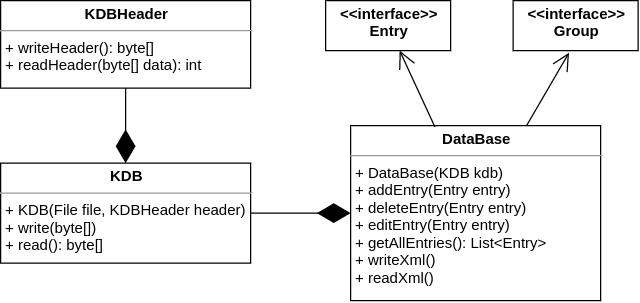
\includegraphics[width=\textwidth]{analysis}
\caption{rappresentazione UML dell'analisi del progetto}
\end{figure}

\chapter{Design}

\section{Architettura}

Per la realizzazione di KeePassJ abbiamo scelto di utilizzare il pattern architetturale
Model-View-Controller (MVC).

TODO: Inserire schema UML MVC.

\section{Design dettagliato}

\section*{Giovanni Di Santi}

Il mio compito principale del progetto è stato quello di gestire la parte crittografica e
definire la struttura dell'header del database. 
Prima di iniziare a modellare le varie parti mi sono documentato sulle tecnologie attuali dei vari keepass,
il paper più citato è "On The Security of Password Manager Database Formats" \cite{security}.
Mi sono ispirato a come funziona il formato di keepass2 \href{https://keepass.info/help/kb/kdbx_4.html}{KDBX4}.
Il formato è composta da un \textit{header} e un \textit{body}.
Nell'\textit{header} sono definiti i vari cipher, kdf, e parametri per cifrare/decifrare
il \textit{body}. Il body decifrato in KDBX4 è formato da un XML, tuttavia questa parte è ha scelta
di chi deve implementare il database in chiaro. Nel nostro caso Massimiliano ha
deciso di usare XML perché ha una buona interoperabilità con Java.

La sezione del paper \textit{4.6} evidenzia come il formato KDBX4 di keepass2 sia
insicuro contro attacchi del tipo \textbf{MAL-CDBA}. Senza entrare nei dettagli,
l'header del database non viene autenticato e quindi si aprono una serie di possibili
attacchi teorici.
Tuttavia il paper sopra citato non è coerente con il sito di keepass2 in cui si descrive
\href{https://keepass.info/help/kb/kdbx_4.html}{KDBX4}, infatti leggendo il sorgente di
keepass2 si può notare che l'autenticazione viene eseguita. Probabilmente il paper
essendo del 2012 non è aggiornato sui recenti cambiamenti.

\subsection*{CryptoCipher}

\textbf{CryptoCipher} è l'interfaccia che descrive i metodi necessari per effettuare
l'encryption e la decryption di un array di \texttt{byte}.\\
Ogni implementazione disponibile di questa interfaccia è un
AEAD Cipher \cite{AEAD}
(Authenticated Encryption with Associated Data).\\
Ho scelto questo schema di encryption per rendere il database resistente ad 
attacchi del tipo \textbf{CCA} (Chosen Ciphertext Attack), cifrando il contenuto del
database e autenticando sia il contenuto che l'header (Associated Data).
\begin{figure}[h]
\centering{}
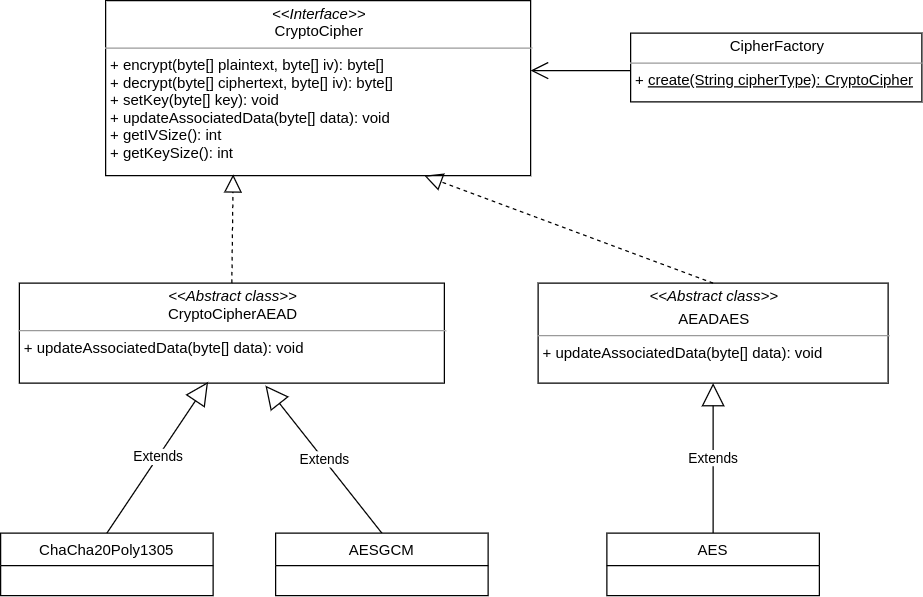
\includegraphics[width=\textwidth]{crypto-cipher}
\caption{rappresentazione UML del pattern factory per creare un CryptoCipher}
\end{figure}
Attualmente i cipher disponibili sono:
\begin{itemize}
  \item ChaCha20-Poly1305 \cite{c20}.
  \item AES-GCM \cite{aesgcm}.
  \item AES-256-CBC-HMAC-SHA-512 \cite{aes}.
\end{itemize}

Esistono due \texttt{abstract class} diverse per implementare un \textbf{CryptoCipher},
poiché la costruzione di \textbf{AES} che sarebbe \texttt{AES-256-CBC-HMAC-SHA-512} è manuale,
mentre \textbf{ChaCha20-Poly1305} e \textbf{AES-GCM} sono implementate direttamente in openjdk11.
La classe astratta \textbf{AEADAES}, permette di essere estesa per costruire altri
cryptosystem come \texttt{AES-192-CBC-HMAC-SHA-384}, tuttavia ho deciso di estendere
solo lo schema più sicuro.\\
Nonostante i dati da cifrare e decifrare sono nella pratica degli \{Input,Output\}Stream,
non ho usato le classi \href{https://docs.oracle.com/en/java/javase/11/docs/api/java.base/javax/crypto/CipherOutputStream.html}{CipherOutputStream}
e \href{https://docs.oracle.com/en/java/javase/11/docs/api/java.base/javax/crypto/CipherInputStream.html}{CipherInputStream}
per:
\begin{itemize}
  \item Rendere più semplice il suo utilizzo.
  \item Facilitare il testing delle varie implementazioni.
\end{itemize}

%Ho usato il design pattern factory per creare un \textbf{CryptoCipher} perché
%quando

\subsection*{KDF}

\textbf{KDF} (Key Derivation Function) è l'interfaccia che descrive i metodi necessari
e opzionali per generare una chiave simmetrica per cifrare/decifrare il database.\\
Gli algoritmi disponibili sono:
\begin{itemize}
  \item Argon2.
  \item Scrypt.
  \item PBKDF2.
\end{itemize}

\begin{figure}[h]
\centering{}
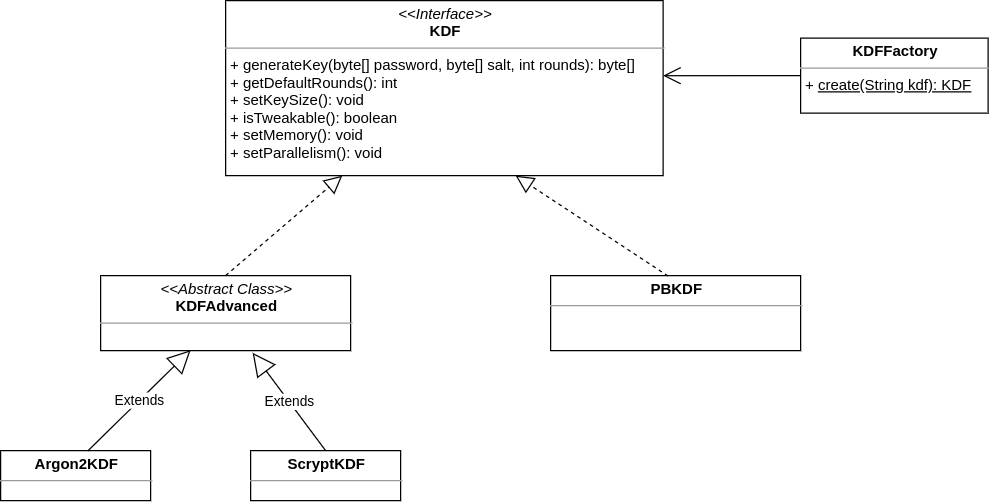
\includegraphics[width=\textwidth]{kdf}
\caption{rappresentazione UML del pattern factory per creare un KDF}
\end{figure}

\textbf{Argon2} e \textbf{Scrypt} estendono \textbf{KDFAdvanced} poiché i loro
algoritmi permettono di definire parametri extra come il paralellismo e la memoria usata
dal KDF. \textbf{PBKDF2} è un vecchio metodo per generare una chiave dalla password e
l'unico parametro configurabile è il numero di round che usa internamente, per questo
ho settato il campo \texttt{tweakable} a falso.

Per capire perché il pattern \texttt{Factory} è usato sia per creare \textbf{KDF}
e \textbf{CryptoCipher} bisogna prima analizzare il parsing dell'header e la relativa
encryption/decryption del database.

\subsection*{KDB}

Per progettare questa parte non ho usato le interfacce perché:
\begin{itemize}
  \item Ho solo una implementazione disponibile.
  \item Sono più flessibile quando devo cambiare la signature di un metodo, senza dover usare un IDE o un LSP per il refactoring.
  \item Principio \href{https://en.wikipedia.org/wiki/You_aren%27t_gonna_need_it}{YAGNI} e \href{https://en.wikipedia.org/wiki/KISS_principle}{KISS}.
\end{itemize}

\textbf{KDBHeader} è la classe che si occupa di:
\begin{itemize}
  \item Parsare l'header (Lettura).
  \item Configurare i vari parametri (Scrittura).
\end{itemize}

\textbf{KDB} è la classe che tramite il \textbf{KDBHeader} si occupa di cifrare/decifrare
dati arbitrari.
Il pattern factory per \textbf{CryptoCipher} e \textbf{KDF} è utile quando in \textbf{KDB}
si effettua l'operazione \texttt{encrypt} e \texttt{decrypt}. I metodi richiedono
a \textbf{KDBHeader} il valore (String) del \texttt{Cipher} e del \texttt{KDF} che viene
passato come parametro di \{Cipher,KDF\}Factory.create() per generare l'oggetto
richiesto.
I due metodi pubblici principali di \textbf{KDB} sono:
\begin{itemize}
  \item \texttt{write}: che esegue l'encryption dell'array di byte in input e lo scrive sul file.
    Ad ogni write viene generato un nuovo IV, che viene poi usato per cifrare il plaintext.
    In questo modo si creano due versioni diverse dello stesso \textit{body} e si rende
    lo schema crittografico sicuro contro vari attacchi di tipo \textbf{CCA}.
  \item \texttt{read}: che legge il file e lo decrypta. Questo metodo lancia un
    \texttt{IOException} se il file non esiste o un \texttt{AEADBadTagException} quando il file è corrotto.
    Il file può risultare corrotto o perché la password è sbagliata o perché è stato effettivamente manipolato.
    Non lancio tipi diversi di eccezioni (es. \texttt{BadPaddingException}) in base a vari tipi di errore,
    per evitare vari tipi di attacchi (praticamente difficili, ma teoricamente possibili) come
    il padding oracle.
\end{itemize}

\begin{figure}[h]
\centering{}
\includegraphics[width=\textwidth]{kdb}
\caption{rappresentazione UML di KDB}
\end{figure}

\section*{Francesco Ercolani}
Il mio ruolo nel progetto KeePassJ è stato quello di sviluppo e gestione dell'interfaccia grafica del programma.
L'interfaccia grafica è gestita attraverso controllers situati nel package \textbf{view.controllers}, ciascuno collegato al rispettivo file fxml presente nella directory \textbf{src/main/resources/view}. 
I controllers utilizzano classi nel package controller per gestire la logica dell'interfaccia.

\subsection*{view.controllers}

Come già citato in precendenza, il package \textbf{view.controllers} contiene tutti i controllers dei rispettivi file fxml; il mio compito è stato quello di creare sia i file fxml che di gestire la logica, con opportuni metodi e campi interni ai rispettivi controllers, di una parte di essi.
La directory src/main/resources/ è gestita nel seguente modo: all'interno della sottodirectory \textbf{/view}, è presente il file \textbf{MainMenu.fxml} e due ulteriori sottodirectory \textbf{/createnew} e \textbf{/database}.
All'interno di /createnew sono presenti i file:
\begin{itemize}
    \item \textbf{chooseNameDb.fxml}: è l'interfaccia per l'inserimento del nome e della descrizione del database.
    \item \textbf{chooseEncryptionSet.fxml}: è l'interfaccia per l'impostazione del metodo di encryption del database.
    \item \textbf{choosePassMenu.fxml}: è l'interfaccia per la scelta della password del database.
\end{itemize}

All'interno di /database sono presenti i file:

\begin{itemize}
    \item \textbf{OpenDatabase.fxml}: è l'interfaccia per l'inserimento della password per l'apertura del database.
    \item \textbf{ManageMenu.fxml}: è l'interfaccia dove vengono visualizzati gli account registrati nel database corrente e dove si può scegliere di aggiungere un account o un gruppo.
    \item \textbf{AddEntry.fxml}: è l'interfaccia dove si aggiungono gli account che si vogliono gestire.
    \item \textbf{AddGroup.fxml}: è l'interfaccia dove si aggiungo i gruppi ai quali apparterranno gli account inseriti.
\end{itemize}

Il file MainMenu.fxml che si trova dentro la directory /view è l'interfaccia principale che viene caricata all'esecuzione del programma e contiene i due pulsanti principali: "Create new database" e "Open database" per appunto rispettivamente creare ed aprire un database. Oltre che della creazione dei file fxml citati, mi sono occupato della creazione di tutti i rispettivi controllers e della gestione della logica interna di essi eccetto per: \textbf{AddEntryController.java}, \textbf{AddNewGroupController.java} e \textbf{ManageMenuController.java} (compito delegato ad altri componenti del gruppo di progetto). \\
Dal controller di MainMenu.fxml \textbf{MainMenuController.java} partono due "linee" separate in riferimento alla creazione o all'apertura di un database. \\
Nel caso si clicchi su "Create new database", la linea prosegue verso il controller dell'interfaccia per l'inserimento del nome e della descrizione del database (chooseNameDb.fxml) \textbf{ChooseNameDBController.java}. Dentro quest'ultimo sono di fondamentale importanza i campi per l'acquisizione dei dati inseriti dall'utente. \\
Cliccando su "Continue" la linea prosegue passando al controller dell'interfaccia adibita al settaggio dell'encryption del database \textbf{ChooseEncrSetController.java}, che a sua volta acquisirà anch'esso i dati inseriti dall'utente.
Continuando con la creazione si arriva all'ultima interfaccia della linea controllata dal controller \textbf{ChoosePassController.java}, il quale alla pressione del bottone "Confirm", attraverso l'oggetto di tipo KDBHeader, setta tutti i valori inseriti dall'utente. \\
La seconda linea invece porta all'interfaccia di inserimento della password per l'apertura del database selezionato in precedenza.\\
\begin{figure}[h]
\centering{}
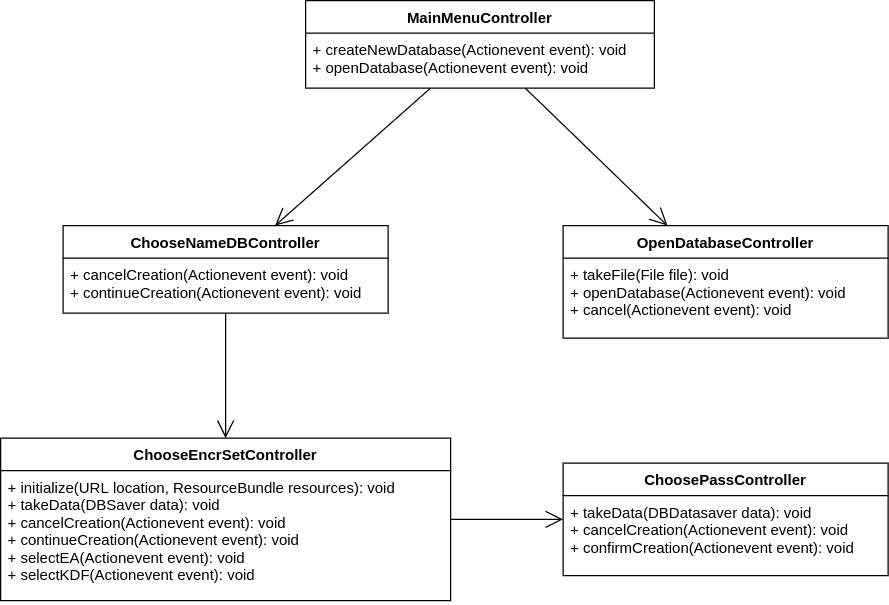
\includegraphics[width=\textwidth]{controllers.png}
\caption{rappresentazione UML delle due linee che collegano i controllers}
\end{figure}\\

I controllers al loro interno hanno un metodo per ciascuna azione che l'utente compie nell'interfaccia.\\ Ciascun controller fa uso di classi presenti nel package \textbf{controller}. Per il loading dei file fxml si utilizza la classe \textbf{FxmlFilesLoaderImpl.java} che implementa la relativa interfaccia \textbf{FxmlFilesLoader.java}.\\
Questa classe ha diversi metodi per fare il caricamento dell'interfaccia in modi differenti: alcuni caricano il file con metodo standard, altri hanno parametri per il passaggio di dati da controller a controller, infatti alcuni controller come da OpenDatabaseController.java in poi, hanno bisogno dei dati inseriti precedentemente.\\
Per implementare questo passaggio ho creato una classe \textbf{DBDataSaverImpl.java} che salva i dati inseriti e li passa, attraverso metodi di FxmlFilesLoaderImpl, al controller successivo. \\
È stato scelto questo approccio per due principali motivi:
\begin{itemize}
    \item In questo modo la conferma e il settaggio dei dati avviene soltanto alla fine del procedimento di creazione.
    \item Il passaggio da controller a controller è più semplice in termini di trasferimento.
\end{itemize}

Ogni controller che richiede dati dal precedente ha quindi un metodo \textbf{takeData()} che prende in ingresso l'oggetto di tipo DBDataSaver.
I controllers utilizzano inoltre la classe \textbf{FxmlSetterImpl.java} che implementa l'interfaccia \textbf{FxmlSetter.java}, per operazioni come:
\begin{itemize}
    \item Settaggio di spinner o warning dialogs.
    \item Acquisizione dello stage corrente.
\end{itemize}

Il settaggio effettivo per la creazione avviene in ChoosePassController.java, alla pressione del pulsante "Confirm" dopo aver scelto il nome e la destinazione del file (deve avere necessariamente l'estensione .kdbj), attraverso le classi KDBHeader e KDB.

Se si sceglie di aprire un database esistente, si apre la schermata di inserimento della password controllata da \textbf{OpenDatabaseController.java} e, in caso di inserimento corretto, si apre la schermata di gestione degli account controllata da \textbf{ManageMenuController.java}.\\
Anche in questo caso il passaggio di dati tra controllers avviene attraverso l'utilizzo della classe \textbf{FxmlFilesLoader}.
\subsubsection*{Vantaggi di questo approccio per il passaggio dei dati:}
\begin{itemize}
    \item Semplicità di utilizzo: è facile passare i dati da un controller all'altro in quanto viene passato soltanto l'oggetto responsabile del raggruppamento di essi.
    \item Non c'è bisogno di settaggi intermedi sugli oggetti KDBHeader e KDB in quanto viene settato tutto alla conferma finale.
\end{itemize}

\clearpage
\begin{figure}[h]
\centering{}
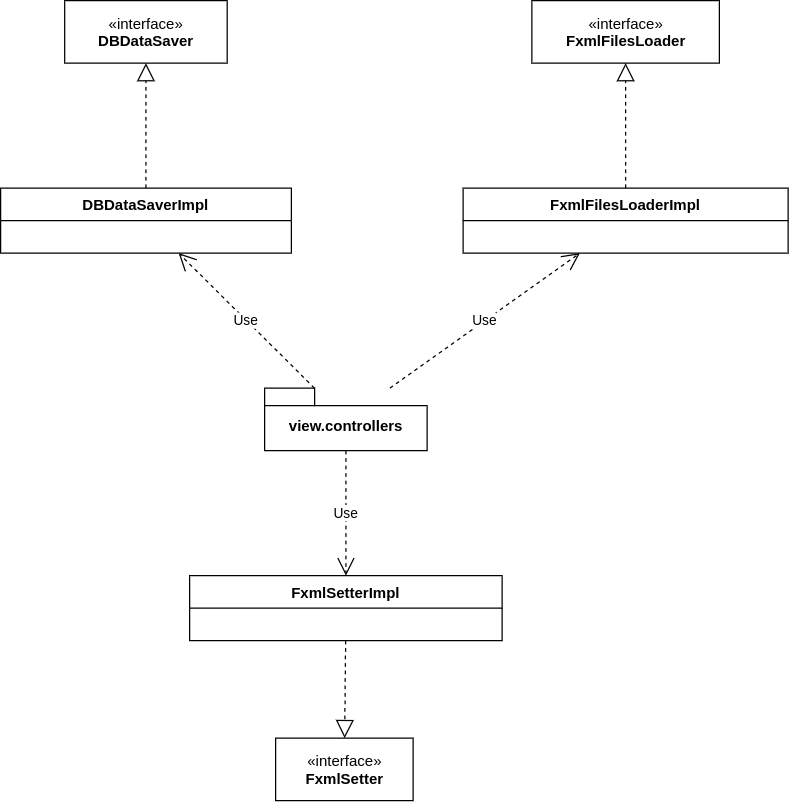
\includegraphics[width=\textwidth]{controller-pkg-view.png}
\caption{rappresentazione UML della relazione tra le classi nel package controller e i controllers in view}

\end{figure}
\subsubsection*{Svantaggi di questo approccio per il passaggio dei dati:}
\begin{itemize}
    \item Ridondanza di codice nella classe FxmlFilesLoaderImpl.
    \item Necessità di modifiche/aggiunte nella classe FxmlFilesLoaderImpl nel caso di cambi/aggiunte di funzionalità nell'applicazione.
\end{itemize}

\subsection*{Esecuzione dell'applicazione}
La classe \textbf{ViewImpl.java} che implementa l'interfaccia \textbf{View.java} nel package view, è incaricata del loading della prima scena del programma.
La classe \textbf{Main.java}, situata all'interno del package \textbf{application}, estende la classe Application di javafx e implementa quindi il metodo \textbf{start()} che è il main entry point dell'applicazione. All'interno del metodo main il programma viene lanciato con il metodo statico \textbf{launch()}.\\
\begin{figure}[h]
\centering{}
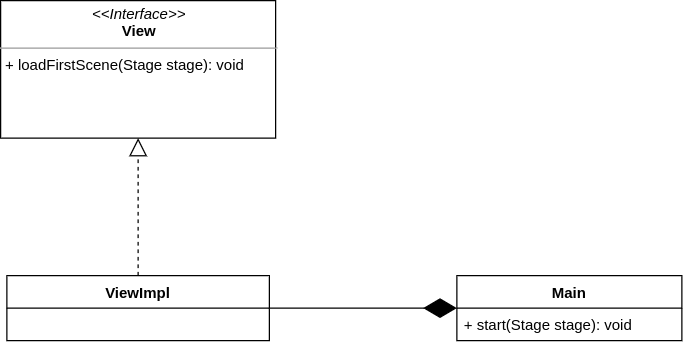
\includegraphics[width=\textwidth]{viewpart.png}
\caption{rappresentazione UML dell'esecuzione dell'applicazione}
\end{figure}


\section*{Massimiliano Conti}

Il mio compito invece è stato di creare e gestire il \textbf{database} e gli elementi contenuti in esso,
tra cui \textbf{Entry} e \textbf{Group} (package \textbf{model.db}), e di convertire il database stesso in un file di tipo XML (package \textbf{model.export}).\\
Per progettare questa parte non ho usato interfacce perchè non erano utili ai fini dell'applicazione implementazioni aggiuntive.\\
In fine ho gestito i \textbf{Controllers} relativi alla visualizzazione del database e relativa
creazione di Entry e Group presenti nel package \textbf{view.controllers}.

\subsection*{Database}

\textbf{Database} è la classe che si occupa di gestire e mantenere i dati inseriti inseriti dall'utente. Contiene i metodi necessari per l'uso e la modifica degli \texttt{ArrayList} usati con relativa creazione ed eliminazione degli oggetti.\\
Oltre a contenere un oggetto String per il mantenimento del nome assegnato e un oggetto KDB (creato da Giovanni).\\

Gli oggeti gestiti dalla classe Database sono:
\begin{itemize}
  \item Entry
  \item Group
\end{itemize}

\textbf{Entry} è la classe su cui si basa il Database perchè con i sui campi nomeAccount, username, password, groupName, url e note mantiene ogni dato che l'utente inserisce riguardo l'account che sta salvando sull'applicazione.\\

\textbf{Group} è la classe adibita alle categorie che l'utente crea o può creare. Ho creato una classe apposita per una più corretta gestione in modo da poter attribuire un nome e anche una descrizione oltre che impedire all'utente nel momento di creazione di una Entry l'inserimento di un nome sbagliato fornendo la lista già presente o la possibilità di creare un nuovo Group. 

\begin{figure}[h]
\centering{}
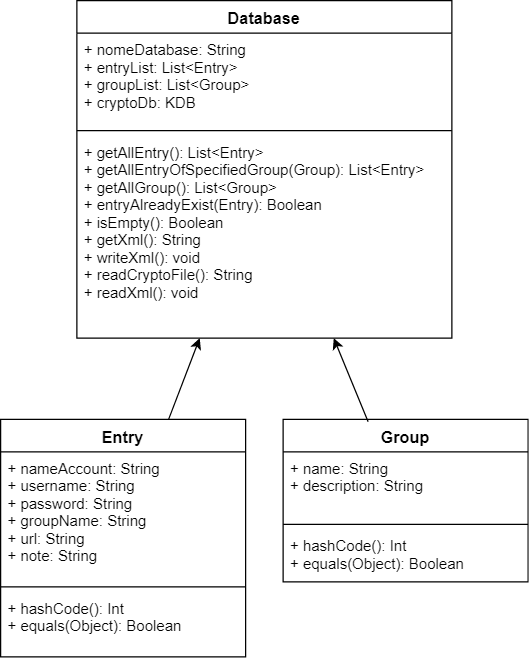
\includegraphics[width=\textwidth]{DatabaseUml}
\caption{rappresentazione UML del Database con Entry e Group}
\end{figure}

\subsection*{ConvertXML}

\textbf{ConvertXML} fa uso della libreria JAXB, architettura per mappare Java objects e documenti XML (\href{https://javaee.github.io/jaxb-v2/}{link to project homepage}.). Questa classe viene usata da due metodi della classe Database, tramite cui creare o recupera dati da un domumento XML.\\

Il funzionamento si basa su due metodi \textit{static}:
\begin{itemize}
  \item toXml
  \item fromXml
\end{itemize}

\textbf{toXml} prende come parametri di input una istanza di Database e con l'uso degli oggetti \texttt{JAXBContext} e \texttt{Marshaller} restituisce in ouput una String contenente un documento XML propriamente riempito con Entries, Groups e il nome del Database.\\

\textbf{fromXml} invece come paramentro di input prende un documento XML contenuto in una String e tramite gli oggetti \texttt{JAXBContext} e \texttt{Unmarshaller} lo converte e crea una nuova istanza della classe Database e la restituisce in output per riempire l'oggetto che ha chiamato la conversione.\\

La classe ha poi un metodo privato \textbf{getTempFile} a cui il metodo fromXml fa appoggio per la creazione di un file usato dall'oggetto Unmarshaller, ma con il vantaggio di non scriverlo fisicamente su disco.\\

\begin{figure}[h]
\centering{}
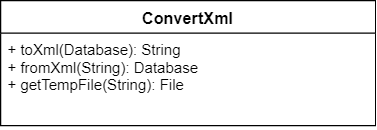
\includegraphics[width=\textwidth]{ConvertXmlUml}
\caption{rappresentazione UML di ConvertXml}
\end{figure}

\subsection*{Controllers}

Mi sono poi occupato di gestire i \textbf{controller} che si occupano di inserire Entry e Group dentro la classe Database e visualizzare i dati.\\
Tra cui:
\begin{itemize}
  \item AddEntryController
  \item AddNewGroupController
  \item ManageMenuController
\end{itemize}

In \textbf{AddEntryController} in particolare ho riempito la ComboBox relativa ai Groups (inseriti tramite \textbf{AddNewGroupController}) e controllato se i campi necessari come Title, username e password non sono vuoti prima di creare una nuova Entry che poi viene inserita nella list dentro Database e poi salvato il file aggiornato.\\(inserimento e controllo della password sono parte di Davide).\\

In \textbf{ManageMenuController} ho creato e riempito le colonne dentro la \textit{TableView} in cui mostro la lista di Entry e la lista di Group.\\Tramite i bottoni è poi possibile eliminare l'Entry selezionata nella tabella e accedere poi alle view di AddEntry e AddGroup.


\section*{Davide Cellot}
\\Il mio compito principale nella realizzazione del progetto è stato quello di gestire la parte legata alle password. Dato che il progetto si basa sul salvataggio di password in database e la loro crittazione, è abbastanza importante gestire in modo ottimale tali password.\\

\\Per prima cosa ho cercato su internet vari siti e applicazioni che inglobavano anche l’inserimento di password e da tali ho preso ispirazione per la creazione del controllo di validità. Dopodiché mi sono concentrato sul calcolo della robustezza (strength) ovvero una misura di efficienza contro eventuali attacchi che una password può subire. Tanto questo numero è più alto, tanto è più sicura la password.\\

\chapter{Sviluppo}
\section{Testing automatizzato}

Durante lo sviluppo del nostro progetto abbiamo utilizzato \texttt{Junit} per
testare il corretto funzionamento delle varie classi.
\textbf{Funzionalità testate automaticamente}:
\begin{itemize}
  \item \textit{CryptoCipher}: viene testato il corretto comportamento dei vari cipher utilizzando lo specifico \texttt{Factory}.
  \item \textit{KDF}: vengono testate le varie KDF utilizzando lo specifico \texttt{Factory}.
  \item \textit{Crypto Util}: test di varie utility per crittografia, come il PKCS\#7 padding e SHA256.
  \item \textit{KDBHeader}: viene testato il corretto funzionamento del \textbf{KDBHeader}, settando vari parametri e controllando il corretto funzionamento dei getter.
  \item \textit{KDB}: test sulla scrittura e lettura di diverse combinazioni di \texttt{cipher} e \texttt{KDF}.
  \item \textit{Database}: viene controllato la corretta creazione ed uso delle liste usate e dei relativi getter.
  \item \textit{Entry}: test sui getter e setter.
  \item \textit{ConvertXml}: test sulla corretta conversione di un Database sample da e verso xml.
\end{itemize}

I test vengono eseguiti anche in remoto tramite l'apposita \texttt{bitbucket pipelines} che
esegue la build del progetto e lancia i vari test.

\section{Metodologia di lavoro}

TODO.

\section{Note di sviluppo}

\section*{Giovanni Di Santi}

\begin{itemize}
  \item \textit{javax.crypto e java.security}: usata per lavorare con Cipher, KDF, e MessageDigest.
  \item \textit{Stream}: usata per manipolare l'header in modo efficace ed elegante.
  \item \textit{Libreria Google Guava}: lavorare con i byte array in java non è comodo. Questa libreria ha varie classi per semplificare
    il lavoro tra cui \href{https://guava.dev/releases/19.0/api/docs/com/google/common/primitives/Bytes.html}{Bytes}.
  \item \textit{ByteBuffer}: per convertire in little endian i bytes, i Data\{Input,Output\}Stream in java lavorano solo in big-endian.
  \item \textit{Libreria Argon2 e Scrypt}: Questi due KDF non erano disponibili dentro \texttt{javax.crypto}.
  \item \textit{Libreria Apache Commons}: per convertire byte array in formato esadecimale.
\end{itemize}

Ho iniziato lo sviluppo leggendo i sorgenti di keepass2, keepassxc e di \href{https://github.com/libkeepass/pykeepass}{pykeepass}.
Non ho trovato librerie simili a \href{https://construct.readthedocs.io/en/latest/index.html}{construct} in
java per parsare l'header utilizzando un linguaggio dichiarativo. L'unica alternativa
era \href{http://kaitai.io/}{kaitai.io}, ma il supporto a java era limitato.
Avendo avuto esperienze con le librerie crittografiche in python e C,
il passaggio a java non è stato difficile.
Per i pattern progettuali ho consultato il materiale didattico e online, ho trovato
che il pattern factory mi aiutasse a risolvere vari tipi di problemi per la generazione
automatica di oggetti e l'ho usato.

\section*{Francesco ercolani}
In quanto incaricato di sviluppare la maggior parte dell'interfaccia grafica dell'applicazione, ho fatto un largo uso della libreria esterna \textbf{JavaFX}, in particolare dei moduli:
\begin{itemize}
    \item \textbf{javafx.controls}: per la gestione dei componenti grafici.
    \item \textbf{javafx.base}: per la gestione degli elementi logici (proprietà, collezioni, eventi ecc...).
    \item \textbf{javafx.fxml}: per la gestione dei file FXML.
\end{itemize}

\section*{Massimiliano Conti}
Nella gestione del Database non ho fatto uso di particolari librerie, anzi ho cercato di usare dove potevo l'interfaccia degli stream.\\
In oltre ho imparato ad usare:
\begin{itemize}
    \item \textbf{JAXB}: in quanto utile nella mia parte di parsing di documenti xml.
    \item \textbf{FXML}: per delle modifiche minori alle view di Database e dati.
    \item \textbf{javafx.fxml}: per la gestione dei controller relativi a Database, Entry e Group.
\end{itemize}

\chapter{Commenti finali}

\section{Autovalutazione e lavori futuri}

\subsection*{Giovanni Di Santi}

L'idea iniziale del progetto è stata mia perché mi piace lavorare con la crittografia.
Mi è piaciuto come ho realizzato la parte di \textbf{CryptoCipher}, tuttavia l'architettura
che riguarda \textbf{KDF} non mi sembra eccellente. Un difetto che ho trovato
è stata l'integrazione manuale dei vari metodi in \textbf{KDF} dentro gli accessor
method di \textbf{KDBHeader}.  Dovrebbero esistere librerie, plugin o pattern di
programmazione su misura per quel tipo di problema ma non li ho usati.
In \textbf{KDB} non ho aderito al Single-responsibility principle (SRP) per comodità,
infatti la classe effettua sia la \texttt{write} che la \texttt{read}, al posto di suddividere
i compiti in due classi diverse. L'ho fatto principalmente perché entrambi i metodi
usano lo stato dell'oggetto (campi) per essere eseguiti, quindi era molto conveniente
tenerli all'interno della stessa classe.

\subsection*{Francesco Ercolani}
Il mio ruolo all'interno del progetto KeePassJ è stato più difficile di quanto mi aspettassi. 
Le interfacce da me create sono molto basiche in quanto la mia esperienza con la librearia JavaFX era nulla, 
e per questo spero di trovare il tempo per proseguire lo sviluppo estetico su un branch personale. 
La gestione logica dei controller non è ottimale in quanto fa uso di classi da me create che contengono codice ridondante. 
L'applicazione in sè è abbastanza "povera" di grafica in quanto priva di diverse funzionalità presenti invece in password manager attualmente in commercio.
Il progetto è molto valido, le applicazioni password manager sono estremamente utili e ricoprono una grande 
responsabilità nel mantenimento in sicurezza dei propri dati personali, ed è per questo che ne sono stato entusiasta fin dall'inizio quando mi è stato proposto come idea da Giovanni Di Santi.
Lo sviluppo di questo processo, nonostante i problemi riscontrati, mi ha fatto trovato la voglia di progettare un'applicazione da zero
 e, allo stesso tempo, come già detto, spero in futuro di ritagliarmi uno spazio per proseguire lo sviluppo di KeePassJ.

\section{Difficoltà incontrate e commenti per i docenti}

\subsection*{Giovanni Di Santi}

Ho dovuto lavorare di più del dovuto perché i miei compagni fino a settembre
non hanno implementato nessuna parte di codice significativo.
A inizio giugno la modellazione e l'implementazione della maggior parte del mio
compito erano completate, tuttavia mi sono ritrovato ad aggiungere parti di 
codice in più a settembre, poiché i miei compagni hanno iniziato a lavorare
solo in quel mese. Vari problemi sarebbero nati subito se avessimo lavorato
insieme. Ad esempio ho dovuto aggiungere vari metodi che aiutassero Francesco a modellare
la GUI, difatti tutti i miei commit di settembre sono getter e setter aggiuntivi.
Avendo progettato l'architettura abbastanza bene non ho avuto problemi ad aggiungere
quelle parti di codice, tuttavia ho dovuto riprendere in mano un codice scritto 3 mesi
prima e continuare a lavorarci sopra. Avrei preferito consegnare con la deadline C.

L'intenzione iniziale quando ho inziato a lavorare sul progetto era di renderlo
compatibile con KDBX4, tuttavia ho notato dopo le prime 15 ore che quel formato
è molto complicato da implementare. Non esiste documentazione del formato e quindi
ho speso molto tempo a reverse ingegnerizzare il codice originale. Dopo le prime ore
di implementazioni ho mantenuto la struttura, ma ho deciso di usare nuovi schemi
crittografici. Non mi sono pentito della scelta fatta poiché mi ha reso più creativo.

\subsection*{Francesco Ercolani}
L'architettura del progetto è rimasta molto vaga per i primi mesi dopo l'avvio del progetto. 
Inizialmente le funzionalità di KeePassJ dovevano essere tante e questo ha suscitato in me 
da subito perplessità riguardo al fatto di riuscire a sviluppare un software con così tante 
features complesse in poco tempo.
Inoltre la situazione Covid, e quindi l'impossiblità di vedersi fisicamente, ha creato all'
interno del gruppo diverse difficoltà di comunicazione dovute a problemi tecnici e/o personali.
L'inizio dello sviluppo è partito in momenti diversi da parte dei componenti e la mancanza di 
collaborazione e di specifiche su come si dovessero svolgere le parti assegnate ha creato ulteriori difficoltà di comprensione.
Personalmente ritengo che fino al mese di agosto ci sia stata troppa poca collaborazione e 
troppo poco impegno nel delineare \textbf{chiaramente} quali fossero \textbf{concretamente} 
le parti software da sviluppare.
Mi prendo le mie responsabilità per il ritardo di consegna della mia parte, ma ritengo che 
parte dei problemi siano nati da situazioni che non dipendono da me o dagli altri componenti del gruppo.
Tuttavia nel complesso reputo che il lavoro svolto sia comunque molto buono data 
l'inesperienza progettuale e di linguaggio comune a tutti e 4.

\appendix
\chapter{Guida utente}

Capitolo in cui si spiega come utilizzare il software. Nel caso in cui il suo uso sia del tutto 
banale, tale capitolo può essere omesso.
%
A tal riguardo, si fa presente agli studenti che i docenti non hanno mai utilizzato il software 
prima, per cui aspetti che sembrano del tutto banali a chi ha sviluppato l'applicazione possono non 
esserlo per chi la usa per la prima volta.
%
Se, ad esempio, per cominciare una partita con un videogioco è necessario premere la barra 
spaziatrice, o il tasto ``P'', è necessario che gli studenti lo segnalino.

\subsection*{Elementi positivi}

\begin{itemize}
 \item Si istruisce in modo semplice l'utente sull'uso dell'applicazione, eventualmente facendo uso di schermate e descrizioni.
\end{itemize}

\subsection*{Elementi negativi}
\begin{itemize}
 \item Si descrivono in modo eccessivamente minuzioso tutte le caratteristiche, anche minori, del software in oggetto.
 \item Manca una descrizione che consenta ad un utente qualunque di utilizzare almeno le funzionalità primarie dell'applicativo.
\end{itemize}

\bibliographystyle{plain}
\bibliography{paper}

\end{document}

